\section{Maximum entropy state}

\begin{frame}{Quantum maximum entropy state}
    \begin{columns}
        \begin{column}{0.5\textwidth}
            Maximum entropy estimate can be extended to quantum mechanics. Given a set observables $\hat{G}_{i}$ it is possible to construct a maximum entropy state as
            \begin{equation*}
                \varrho_{max}=\frac{1}{\Tr(e^{\sum_{i}\lambda_{i}\hat{G}_{i}})}e^{\sum_{i}\lambda_{i}\hat{G}_{i}},
            \end{equation*}
            where $\lambda_{i}$ are the Lagrange multipliers used to maximize the von Neumann entropy
            \begin{equation*}
                S(\rho)=-\Tr(\rho\ln{\rho}).
            \end{equation*}
        \end{column}
        \begin{column}{0.5\textwidth}
            Because we're dealing with a coarse grained system, we do not have acces to all the observables of the system. Our coarse graining map
            \begin{equation*}
                \CG{\varrho}=\Tr_{2}(p\varrho+(1-p)S\varrho S^{\dag})
            \end{equation*}
            is of the form $\mcC:\mcS(\hilbert_{4})\rightarrow\mcS(\hilbert_{2})$. Meaning we have access to a tomographically complete set of observables in $\mcS(\hilbert_{2})$. 
        \end{column}
    \end{columns}
\end{frame}

\begin{frame}{State construction}
    \begin{columns}
        \begin{column}{0.5\textwidth}
            If we use the Pauli spin observables, $\sigma_{i}$:
            \begin{align*}
                \langle \sigma_{i}\rangle=&\Tr{\sigma_{i} \rho}\\
                =&\Tr{\sigma_{i}\otimes\Id(p\varrho+(1-p)S\varrho S)}\\
                =&\Tr{(p\sigma_{i}\otimes\Id+(1-p)\Id\otimes\sigma_{i})\varrho}\\
                =&\Tr{\hat{G}_{i}\varrho}\\
                =&\langle \hat{G}_{i}\rangle.
            \end{align*}
            We can construct $\varrho_{max}$ via
            \begin{equation*}
                \hat{G}_{i}=p\sigma_{i}\otimes\Id+(1-p)\Id\otimes\sigma_{i}.
            \end{equation*}
        \end{column}
        \begin{column}{0.5\textwidth}
            Maximum entropy state is
            \begin{equation*}
                \varrho_{max}(\rho)=\frac{1}{Z}\text{exp}(-\sum_{i}\lambda_{i}\hat{G}_{i}).
            \end{equation*}
            But may be written as
            \begin{equation*}
                \varrho_{max}=\frac{e^{-\lambda p(\hat{r}_{\rho}\cdot\vec{\sigma})}}{Z_{1}} \otimes \frac{e^{-\lambda(1-p)(\hat{r}_{\rho}\cdot\vec{\sigma})}}{Z_{2}}.
            \end{equation*}
            Where $\hat{r}_{\rho}$ is $\rho$'s unit Bloch vector, and $\lambda=\sqrt{\lambda^{2}_{1}+\lambda^{2}_{2}+\lambda^{2}_{3}}$.
        \end{column}
    \end{columns}
\end{frame}


\begin{frame}{Lagrange \textit{variable} and purity}
    \begin{columns}
        \begin{column}{0.5\textwidth}
            Having $\varrho_{max}$ in terms of $\lambda$ instead of observables is not ideal. The effective state is
            \begin{equation*}
                \rho=\frac{1}{2}(\Id+r_{\rho}\hat{r}_{\rho}\cdot\vec{\sigma}).
            \end{equation*}
            The relation between the observables and the Lagrange variable is
            \begin{equation*}
                r_{\rho}=-(p\tanh{\lambda p}+(1-p)\tanh{\lambda (1-p)}).
            \end{equation*}
            $r_{\rho}$ is realted to purity of the effective state by
            \begin{equation*}
                r_{\rho}=\sqrt{2\text{Pu}(\rho)-1}.
            \end{equation*}
        \end{column}
        \begin{column}{0.5\textwidth}
            \begin{figure}[h!]
                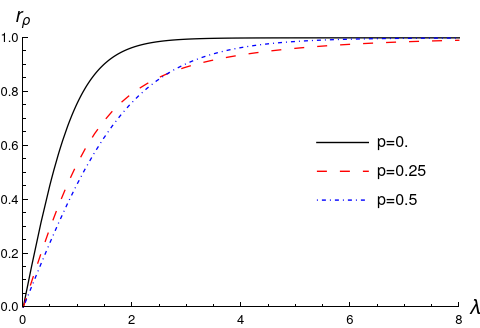
\includegraphics[width=0.8\columnwidth]{figures/r(lambda).png}%
                \caption{$r_{\rho}$ as a function of $\lambda$ for different values of $p$}
            \end{figure}
        \end{column}
    \end{columns}
\end{frame}
